\section{Rendezvous and Docking Constraints} \label{sec:constraints}
%% This section predominantly focuses on the addition of time-varying collision constraints and time-varying final states that are deterministic for the sake of this paper.
\subsection{Time-Varying Final State Constraint}
\label{sec:time-varying-final-state-constraint}
Although the docking position is fixed relative to the target, it is rotating in the LVLH frame.
As a result, we incorporate a time-varying final state heuristic $\zeta(\boldsymbol{r}(\theta_f))$ such that the chaser tracks and attaches to the target at a set docking point.
The upper bound of this heuristic is decreased sequentially in the rendezvous operation to emulate observation spheres.
On the other hand, to facilitate docking, this heuristic is set to zero for docking.
Let the desired docking point be represented as $\left.\boldsymbol{\rho}_{\theta_f,T}\right|_{\theta_T=0}$ for when the target is at no rotation.
The final state heuristic can be defined using the Newton-Euler equations as follows:
\begin{align}
    \boldsymbol{\theta}_T(\theta)&=\begin{bmatrix}\alpha_T(\theta)&\beta_T(\theta)&\gamma_T(\theta)\end{bmatrix}\\
    \dot{\boldsymbol{\theta}}_T(t)&=\boldsymbol{\omega}_T(t)\\
    I\dot{\boldsymbol{\omega}}_T(t)&=-\boldsymbol{\omega}_T(t)\times I\boldsymbol{\omega}_T(t) + \boldsymbol{\tau}_T(t)\\
    % {\mathcal{R}}(\theta)&=\begin{bmatrix}
        % c\beta c\gamma & - c\beta s\gamma & s\beta \\
        % c\alpha s\gamma + s\alpha s\beta c\gamma & c\alpha c\gamma - s\alpha s\beta s\gamma & - s\alpha c\beta \\
        % s\alpha s\gamma - c\alpha s\beta c\gamma & s\alpha c\gamma + c\alpha s\beta s\gamma & c\alpha c\beta 
    % \end{bmatrix}\\
    \zeta(\boldsymbol{r}(\theta_f))&=\boldsymbol{r}(\theta_f)-\left.R(\theta_f)\boldsymbol{\rho}_{\theta_f}\right|_{\theta_T=0}
\end{align}
% where $c(\cdot)=\cos(\cdot)$, $s(\cdot)=\sin(\cdot)$, $\alpha=\alpha_T(\theta)$, $\beta=\beta_T(\theta)$, $\gamma=\gamma_T(\theta)$ (for the rotation matrix only),
where $R(\theta_f)$ is the rotation matrix at the final true anomaly $\theta_f$, $\boldsymbol{\tau}_T(t)=0$ until the end of docking, and time $t$ and true anomaly $\theta$ are interchangeable using the relations given in Section \ref{sec:relevant-knowledge}.\\
Now, for rendezvous, we bound this final state heuristic by a positive "radius" since it is not feasible to reach the final state while operating under the time-invariant rendezvous collision constraint (explained in Section \ref{sec:rendezvous-collision-constraints}).
This gives us the final state cost for rendezvous as follows:
\begin{equation}
    h(\boldsymbol{r}(\theta_f))|_{\text{rend}}=Q_\text{rend}\max{\left(||\zeta(\boldsymbol{r}^P(\theta_f))||-r_R, 0\right)}
\end{equation}
For docking, we define the final state cost so that this heuristic approaches zero at the final true anomaly:
\begin{equation}
    h(\boldsymbol{r}(\theta_f))|_{\text{dock}}=Q_\text{dock}\zeta(\boldsymbol{r}^P(\theta_f))
\end{equation}
\subsection{State and Input Bounds}
\label{sec:state-input-bounds}
Given the general definition for state and input bounds, \cite{brett2019dynamic}
\begin{align}
    ||P_{\boldsymbol{r}}\boldsymbol{r}(\theta)+q_{\boldsymbol{r}}||&\leq C_{\boldsymbol{r}}\\
    ||P_{\boldsymbol{u}}\boldsymbol{u}(\theta)+q_{\boldsymbol{u}}||&\leq C_{\boldsymbol{u}},
\end{align}
we define the following bounds:
% \begin{align}
%     ||\boldsymbol{r}^P(t)||_\infty&<    \infty,\quad\text{(no bound)}\\
%     ||\boldsymbol{r}^V(t)||_\infty&\leq C_{\boldsymbol{r}^V},\\
%     ||\boldsymbol{u}  (t)||_\infty&\leq C_{\boldsymbol{u}}
% \end{align}
\begin{align}
    |r_i^P(\theta)|&<    \infty,\quad\text{(no bound)}\\
    |r_i^V(\theta)|&\leq C_{V},\\
    |u_i  (\theta)|&\leq C_{u},
\end{align}
for each dimension $i=1,2,3$, where $C_{V}$ and $C_{u}$ are constants.
\subsection{Rendezvous Collision Constraints}
\label{sec:rendezvous-collision-constraints}
We define rendezvous to be necessarily bounded outside the positional limits of the target.
As a result, we constrain the chaser from entering a minimal sphere that completely bounds the target.
Since the sphere is a cyclically symmetrical shape in all directions, the rotation of the target does not affect its shape or size and, hence, the constraint is time-invariant, hence reducing computational complexity for the rendezvous problem.
Therefore, the rendezvous collision constraint can be written as follows:
\begin{align}
    {\mathcal{C}}_R:\{\boldsymbol{r}:||\boldsymbol{r}||&>\rho_T\}\\
    \rho_T&=\min\{\rho:||\boldsymbol{p}_T||<\rho\ \forall\ \boldsymbol{p}_T\in\text{T}\}
\end{align}
where T represents the set of points on the target that minimally defines the complete boundary of the target.\\
Alternatively, the constraint can be described by the minimum enclosing ellipsoid of the target (Refer to Appendix \ref{app:mee}) to minimize the distance between the chaser and the target prior to docking.
Although this demands some information regarding the shape and rotation of the target, it can be observed that some amount of symmetry can be used to reduce complexity using such a constraint.
\subsection{Time-Varying Docking Collision Constraints}
\label{sec:time-varying-collision-constraints}
\begin{figure}[htb]
    \centering
    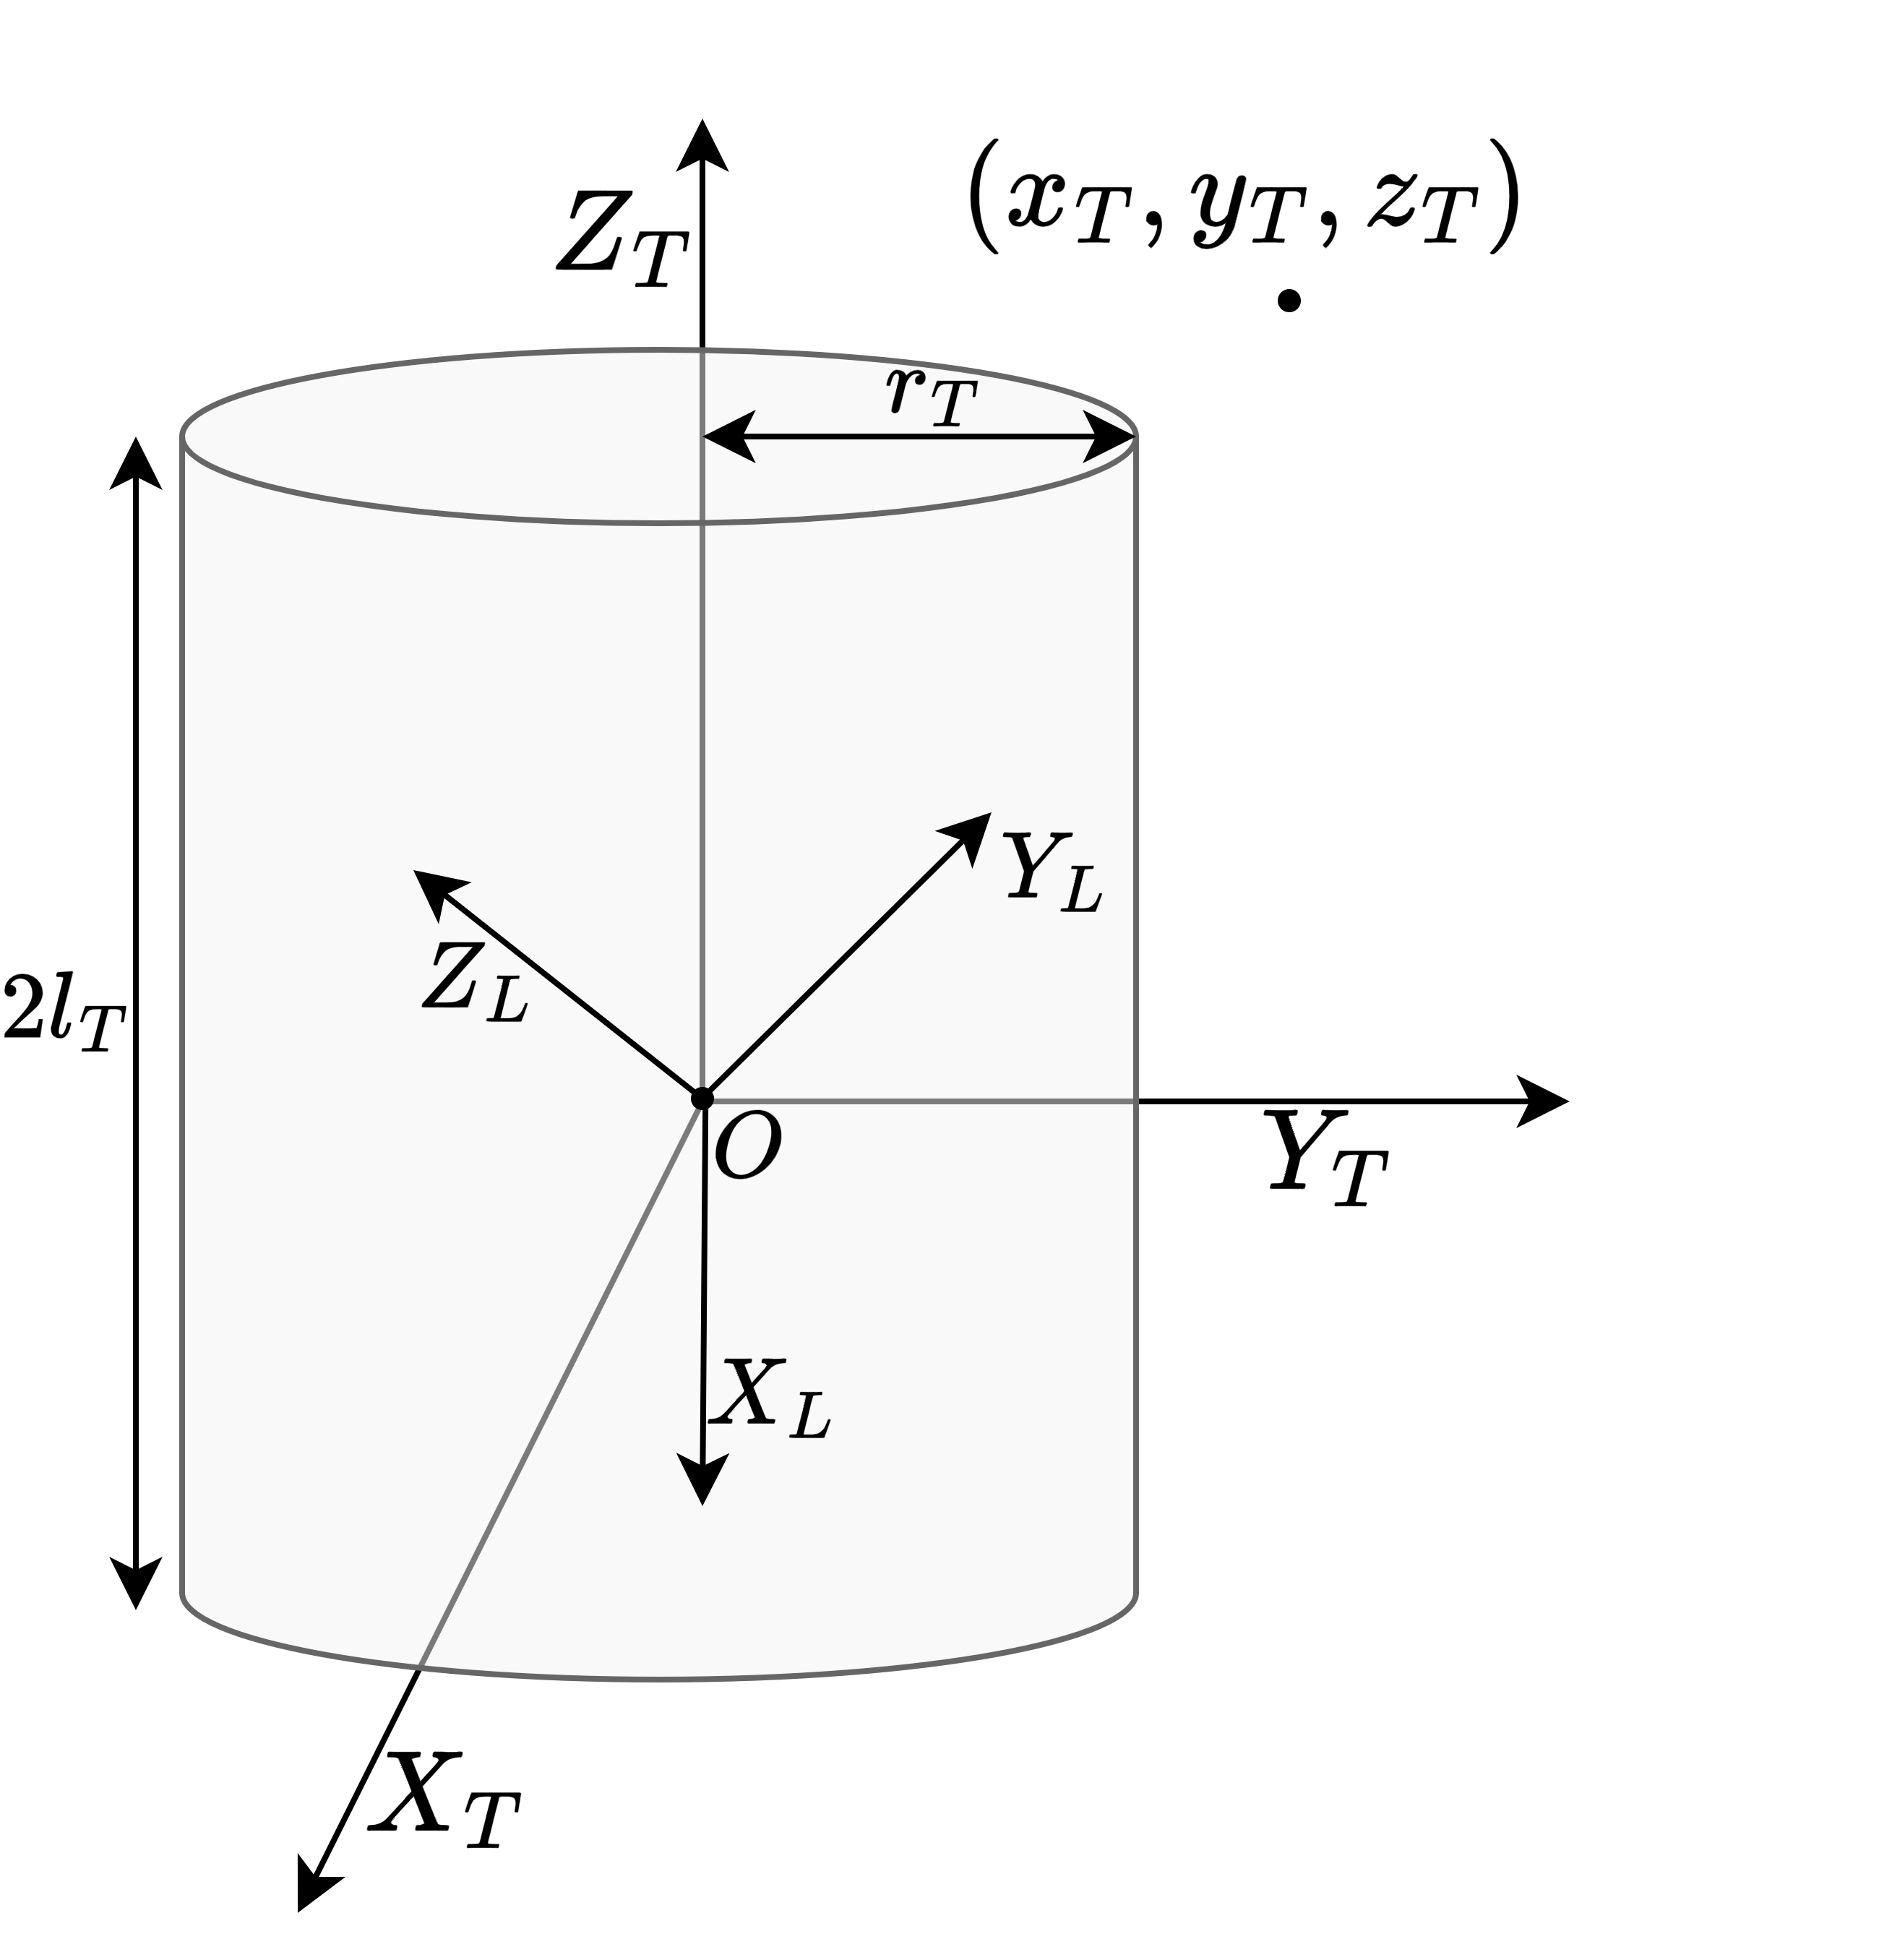
\includegraphics[width=0.9\linewidth]{assets/target-cylinder.png}
    \caption{\textbf{Frames of Reference centered at the Target}: The axes subscripted by $T$ belong to the body frame of the target that rotates with the target and the axes subscripted by $L$ belong to the local-vertical-local-horizontal (LVLH) frame that is defined in Section \ref{sec:relevant-knowledge}}
    \label{fig:target-cylinder}
\end{figure}
The docking operation involves a tighter time-varying state constraint to prevent collisions between the chaser and the target while permitting docking to the boundary of the target.
The same rotational characteristics of the target described in Section \ref{sec:time-varying-final-state-constraint} introduce time-varying collision constraints for the chaser that can be represented as $\boldsymbol{r}(\theta)\in{\mathcal{C}}_D$.
This is motivated by the concept of exclusion from target space as proposed in \cite{park2017nonlinear}.\\
For instance, if the target is cylindrical with radius $r_T$ and length $2l_T$ centered at the origin as demonstrated in Figure \ref{fig:target-cylinder} and rotates such that its rotation matrix at time $t$ is given as $R(t)$, the permissible state set ${\mathcal{C}}_D$ for the chaser can be written as the following union:
\begin{subequations}\label{third:main}
\begin{align}
    {\mathcal{C}}_D&={\mathcal{C}}_{D1}\cup{\mathcal{C}}_{D2}\label{eqn:or-function}\tag{\ref{third:main}}\\
    {\mathcal{C}}_{D1}&=\{\boldsymbol{r}(\theta):f_{D1}=x_{\mathcal{R}}(\theta)^2 + y_{\mathcal{R}}(\theta)^2 - r_T^2\geq0\}\\
    {\mathcal{C}}_{D2}&=\{\boldsymbol{r}(\theta):f_{D2}=||z_{\mathcal{R}}(\theta)|| - l_T\geq0\}
\end{align}
\end{subequations}
where the de-rotated state vector $r_{\mathcal{R}}(\theta)$ (i.e., the position of the chaser as viewed in a target-centered frame of reference that rotates with the target) is defined as:
\begin{align}
    \boldsymbol{r}_{\mathcal{R}}(\theta)&=\begin{bmatrix}
        x_{\mathcal{R}}(\theta)&y_{\mathcal{R}}(\theta)&z_{\mathcal{R}}(\theta)&\dot{x}_{\mathcal{R}}(\theta)&\dot{y}_{\mathcal{R}}(\theta)&\dot{z}_{\mathcal{R}}(\theta)
    \end{bmatrix}^T\notag\\
    &=\left(R^{-1}(\theta)\otimes I_2\right)\boldsymbol{r}(\theta)
\end{align}
Here, $A\otimes B$ represents the Kronecker product of the two matrices $A$ and $B$.
Also, we recall that ${\mathcal{R}}^{-1}={\mathcal{R}}^T$.
The above union can be implemented on a numerical solver using the following logic:
\begin{align}
    {\mathcal{C}}_D=\{\boldsymbol{r}(\theta)\ |\ \text{sgn}(f_{D1})+\text{sgn}(f_{D2})\geq0\}
\end{align}
% The above union can be implemented on a numerical solver as:
% \begin{align}
%     {\mathcal{C}}_D=\{\boldsymbol{r}(\theta)|\max\{{\mathcal{C}}_{D1}, {\mathcal{C}}_{D2}\}\geq0\}.
% \end{align}
% Alternatively, when the $\max$ function is not available, this can be implemented using the following logic:
% \begin{align}
%     {\mathcal{C}}_D=\{\boldsymbol{r}&(\theta)|\notag\\
%     &f_{D1}f_{D2}\left(\left(f_{D1}+f_{D2}\right)-\left(|f_{D1}|+|f_{D2}|\right)\right)\geq0\}
% \end{align}
% or using the following logic:
% \begin{align}
%     {\mathcal{C}}_D=\{\boldsymbol{r}(\theta)|\text{sgn}(f_{D1})+\text{sgn}(f_{D2})\geq0\}
% \end{align}
% such that the logic presented in Table \ref{tab:or-logic} holds.
% \begin{table*}[t]
%     \centering
%     \begin{tabular}{||c|c||c|c||c||}
%     \hline
%         ${\mathcal{C}}_1$ & ${\mathcal{C}}_2$ & ${\mathcal{C}}_1{\mathcal{C}}_2$ & $({\mathcal{C}}_1+{\mathcal{C}}_2)-(|{\mathcal{C}}_1|+|{\mathcal{C}}_2|)$ & ${\mathcal{C}}={\mathcal{C}}_1{\mathcal{C}}_2\left(\left({\mathcal{C}}_1+{\mathcal{C}}_2\right)-\left(|{\mathcal{C}}_1|+|{\mathcal{C}}_2|\right)\right)$ \\
%     \hline
%         + & + & + & 0 & 0 \\
%         + & - & - & - & + \\
%         - & + & - & - & + \\
%         - & - & + & - & - \\
%     \hline
%     \end{tabular}
%     \caption{Implementation of OR Logic in the Optimization Problem}
%     \label{tab:or-logic}
% \end{table*}